\section{Experiment 2 Results} \label{results-2}
In this section, we first describe the participants' demographic in the second experiment. Then, we present descriptive statistics for the raw data. Lastly, we discuss results from our Bayesian analysis.

\subsection{Participants Demographic}
We collected N complete responses in the second experiment. We removed X poor-quality responses where participants responded the qualitative question facetiously and put the same survey rating across all video elements. Similar to experiment 1, we recruited the participants to match the demographic distribution in the US 2019 census data in terms of age and education level, as shown in \Cref{table:demo_exp2}.

\begin{table}
  \centering
  \caption{Experiment 2 sample demographics statistics align closely with 2019 US census. (To be updated with final data) } \label{table:demo_exp2}
  \sisetup{
    table-number-alignment = center, 
    table-figures-integer = 2, 
    table-figures-decimal = 2,
    round-mode = figures,
    round-precision = 3,
    detect-weight=true
    % mode=text
  } \begin{tabularx}{0.5\textwidth}
    {@{}>{\raggedleft\arraybackslash}X>{\bfseries}SS@{}}
    \toprule
    Demographics & {Sample (\si{\percent})} & {Census (\si{\percent})} \\
    \midrule
    \textsc{\bfseries Education} & &\\
    No High School & 16.07 & 10.22  \\
    High School & 25.00 & 27.73  \\
    College  Associate & 28.57 & 33.09  \\
    Bachelor's Degree and above & 30.36 & 33.09  \\ 
    \textsc{\bfseries Age} & &\\
    18--24 & 21.43 & 13.65  \\
    25--39 & 26.79 & 30.74  \\
    40--54 & 25.00 & 28.32  \\
    55--69 & 26.79 & 27.29  \\
    \bottomrule\end{tabularx}
\end{table}

\subsection{Descriptive Statistics}

As shown in \Cref{fig:likert_exp2} and \Cref{fig:qv3_exp2}, on an aggregated level, participants expressed similar relative preferences across the five video elements in both Likert and QV. Audio quality ranked the highest in both cases, while motion smoothness and audio-video synchronization had the lowest ranks. While the aggregated preference were similar between Likert and QV, we will discuss their differences on an individual level in the next subsection. Similar to experiment 1, a majority of the Likert response distributions were left-skewed; in contrast, QV response distributions approximated a Normal distribution. (add QV budget usage)

\begin{figure}[htpb]
\centering
\begin{minipage}[b]{0.44\linewidth}
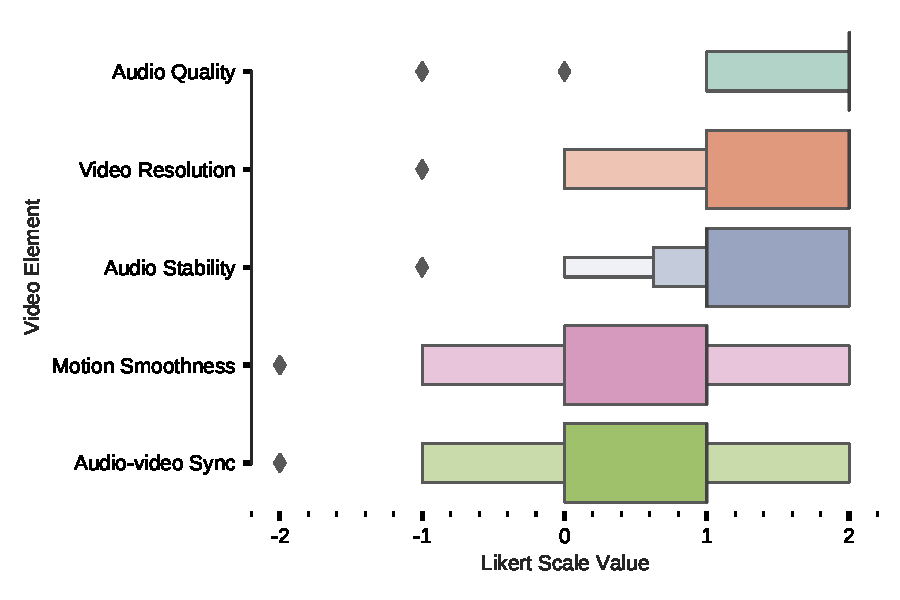
\includegraphics[width=\textwidth, keepaspectratio=true]{content/image/likert_distribution_per_element (1).pdf}
    \caption{
      Distribution of Likert responses per video elements in Boxen plot. 
      Each level from -2 to 2 corresponds to 
      ``Very unimportant'', ``Unimportant'', ``Neutral'', ``Important'', and ``Very important''.
    }
    \Description[Distribution of Likert Responses per element for experiment 2 in Boxen plot]{Distribution of Likert Responses per element for experiment 2 in Boxen plot}
    \label{fig:likert_exp2}
\end{minipage}
\quad
\begin{minipage}[b]{0.52\linewidth}
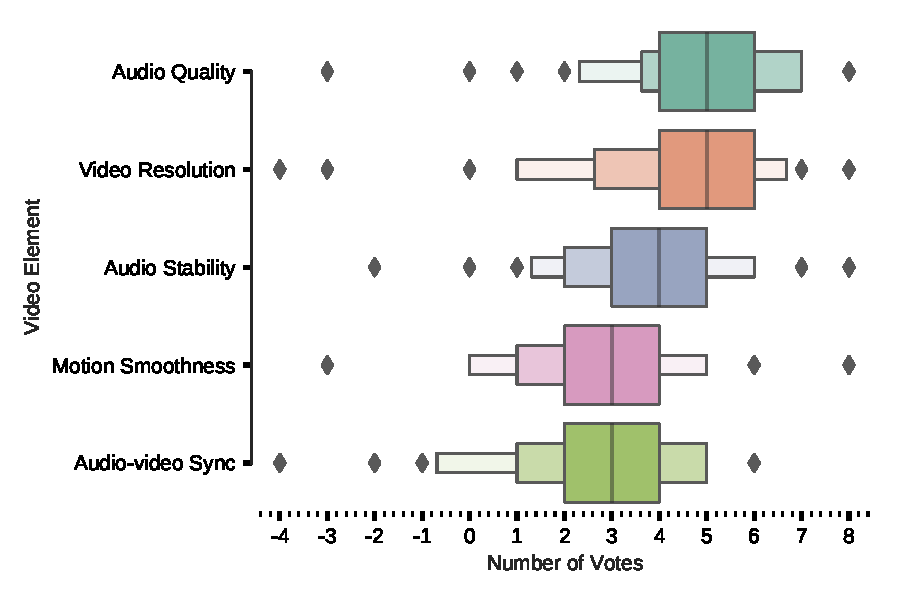
\includegraphics[width=0.9\textwidth, keepaspectratio=true]{content/image/qv_distribution_per_element.pdf}
    \caption{
      Distribution of QV responses per video element in QV in Boxen plots. The maximum possible number of votes on an element was 10 votes given 100 voice credits. Most distributions in all three QV set-ups follow a normal distribution. 
    }
    \Description[Distribution of QV Responses per element for experiment 2]{Distribution of QV Responses per element for experiment 2}
    \label{fig:qv3_exp2}
\end{minipage}
\end{figure}

\begin{figure}[h]
    \centering
    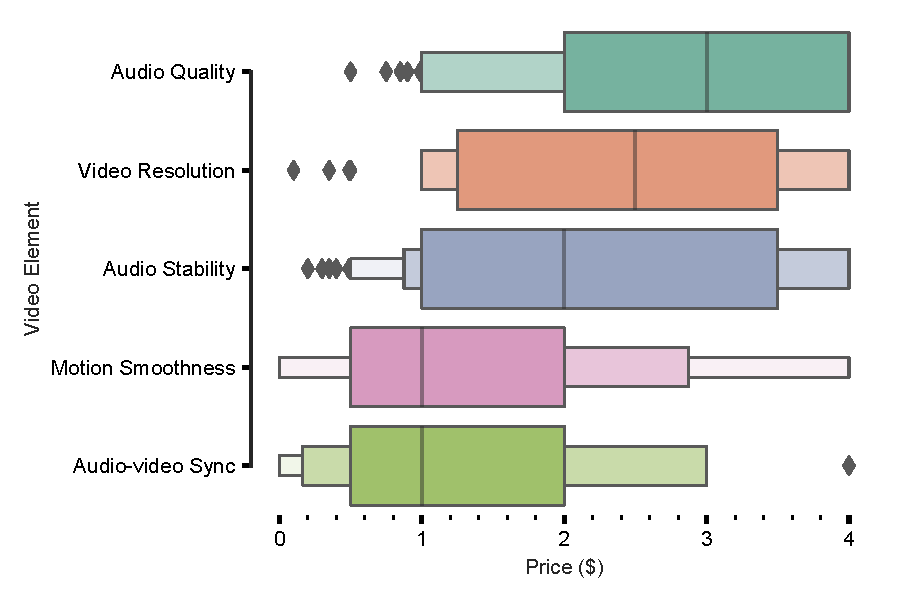
\includegraphics[width=0.5\textwidth, keepaspectratio=true]{content/image/price_distribution_per_element.pdf}
    \caption{
      Distribution of prices set by participants per video elements in Boxen plot. 
      Prices ranged from \$0 to \$4. Compared to the survey response distributions, elements with a higher rating of importance in surveys also had higher prices during product design.
    }
    \Description[Distribution of prices per element in experiment 2 in Boxen plot]{Distribution of prices set for each element in experiment 2 in Boxen plot}
    \label{fig:price_exp2}
\end{figure}


Set prices for the five video elements exhibited similar patterns as the survey responses on an aggregated level (\Cref{fig:price_exp2}). Compared to the survey response distributions, elements with a higher average rating of importance in surveys also had higher average prices during product design. Since we instructed participants during price-setting that the buyer would be willing to pay more for the element that they value more, the alignment of preferences on an aggregated level between surveys and prices indicated that the participants kept our instruction in mind when they decided on the prices.


Similar to experiment 1, we are interested in the degree of alignment between survey responses and prices set in an incentive-compatible scenario on an individual level. \Cref{fig:topic_covariate_exp2} visualizes the estimated correlation between normalized Likert or QV responses and normalized prices. All elements had a trend line with a positive slope, suggesting potential positive correlations. QV responses seemed to had a more positive slope with prices compared to Likert responses, indicating a possibly better alignment. Next, we present statistical support for this phenomenon.

\begin{figure}[htpb]
    \centering
    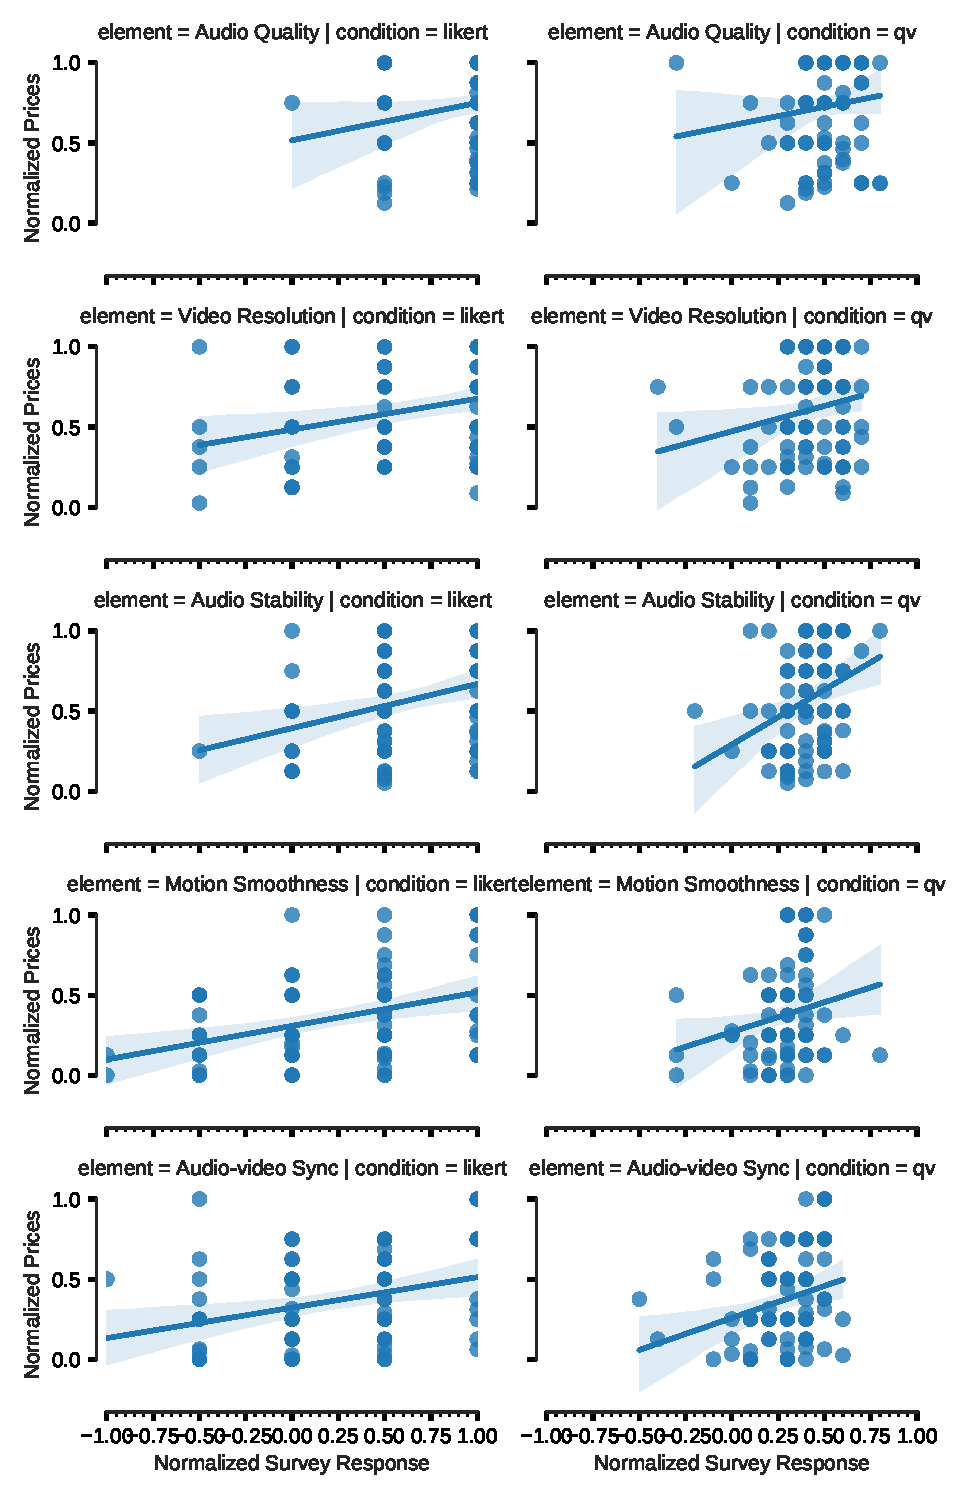
\includegraphics[width=0.6\textwidth, keepaspectratio=true]{content/image/correlation_per_element.pdf}
    \caption{
      Scatterplots showing the correlation between participants' normalized survey response and normalized prices for five video elements in Likert and QV. Each row is one topic, and each column is one survey condition. All elements had a trend line with a positive slope, indicating potential positive correlations.
    }
    \Description[Correlation scatterplots between normalized survey responses and normalized prices for experiment 2]{
      Scatterplots showing the relationship between participants' normalized survey response and normalized prices for each of the five video elements in Likert and QV.
    }
    \label{fig:topic_covariate_exp2}
\end{figure}


\subsection{Bayesian Analysis Results}


\begin{figure}[htpb]
  \centering
  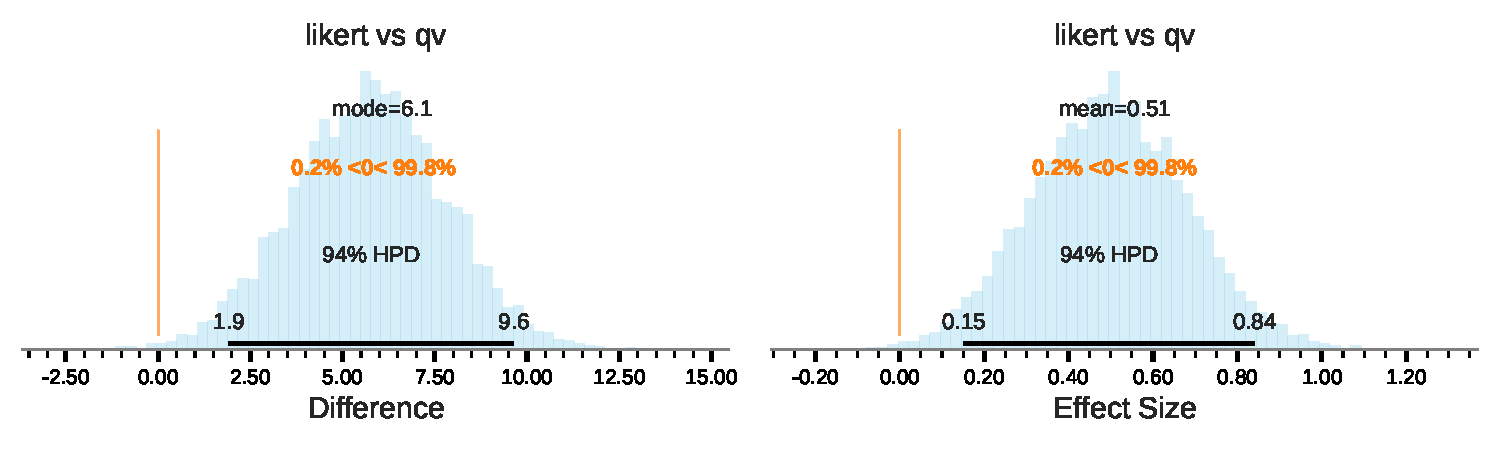
\includegraphics[trim= 0in 0in 0in 0in, clip, width=0.8\textwidth, keepaspectratio=true]{"content/image/Votes_Prices_StudentT_differences_and_effects.pdf"}
  \caption{
    The figure shows the contrasts distribution of the mean Cosine similarity angles between the Likert and QV. The subgraph on the left shows the absolute difference while the one on the right is about the effect size. Since we are highlighting contrasts, each sub-figure shows an orange vertical line located at 0. The main finding is: survey responses from QV aligned significantly better with the price setting behavior than Likert responses with a medium effect size.
  }
  \Description[Contrasts distribution of the mean Cosine similarity angles between Likert and QV for experiment 2]{Contrasts distribution of the mean Cosine similarity angles between Likert and QV for experiment 2}
  \label{fig:contrast_exp2}
\end{figure}

Overall, our Bayesian analysis for experiment 2 showed that QV survey responses aligned significantly better with the price setting behaviors than Likert responses with a medium effect size (0.5 - 0.6). The first graph in the left column of~\Cref{fig:traceplot_exp2}, which contains traceplots for the MCMC estimations, shows that the distribution of the mean Cosine similarity angle for QV (orange line) is to the left of that for Llikert (blue line). Since a perfect alignment means a zero angle, QV had better alignment with the set prices relative to Likert. 

To confirm if the difference was statistical significant, we constructed the distribution of the absolute difference between the means and the distribution of the corresponding effect size (normalized difference), as shown in \Cref{fig:contrast_exp2}. In the subfigure on the left, the mode of the contrast is $6.8$, meaning that the Cosine similarity angles in the Likert group were most frequently $6.8$ degrees larger than the angles in the QV group. Since the HPD of [$2.8$, $11$] lies outside a significant ROPE (Region of Practical Equivalence) of $0 \pm 1 \deg$, there was a significant difference between the alignment levels of the two survey instruments. The medium to high effect size is significant based on the figure on the right, with a modal value of $0.6$ and a HPD interval of [$0.25$, $0.98$].


\begin{sidewaysfigure*}
  \centering
  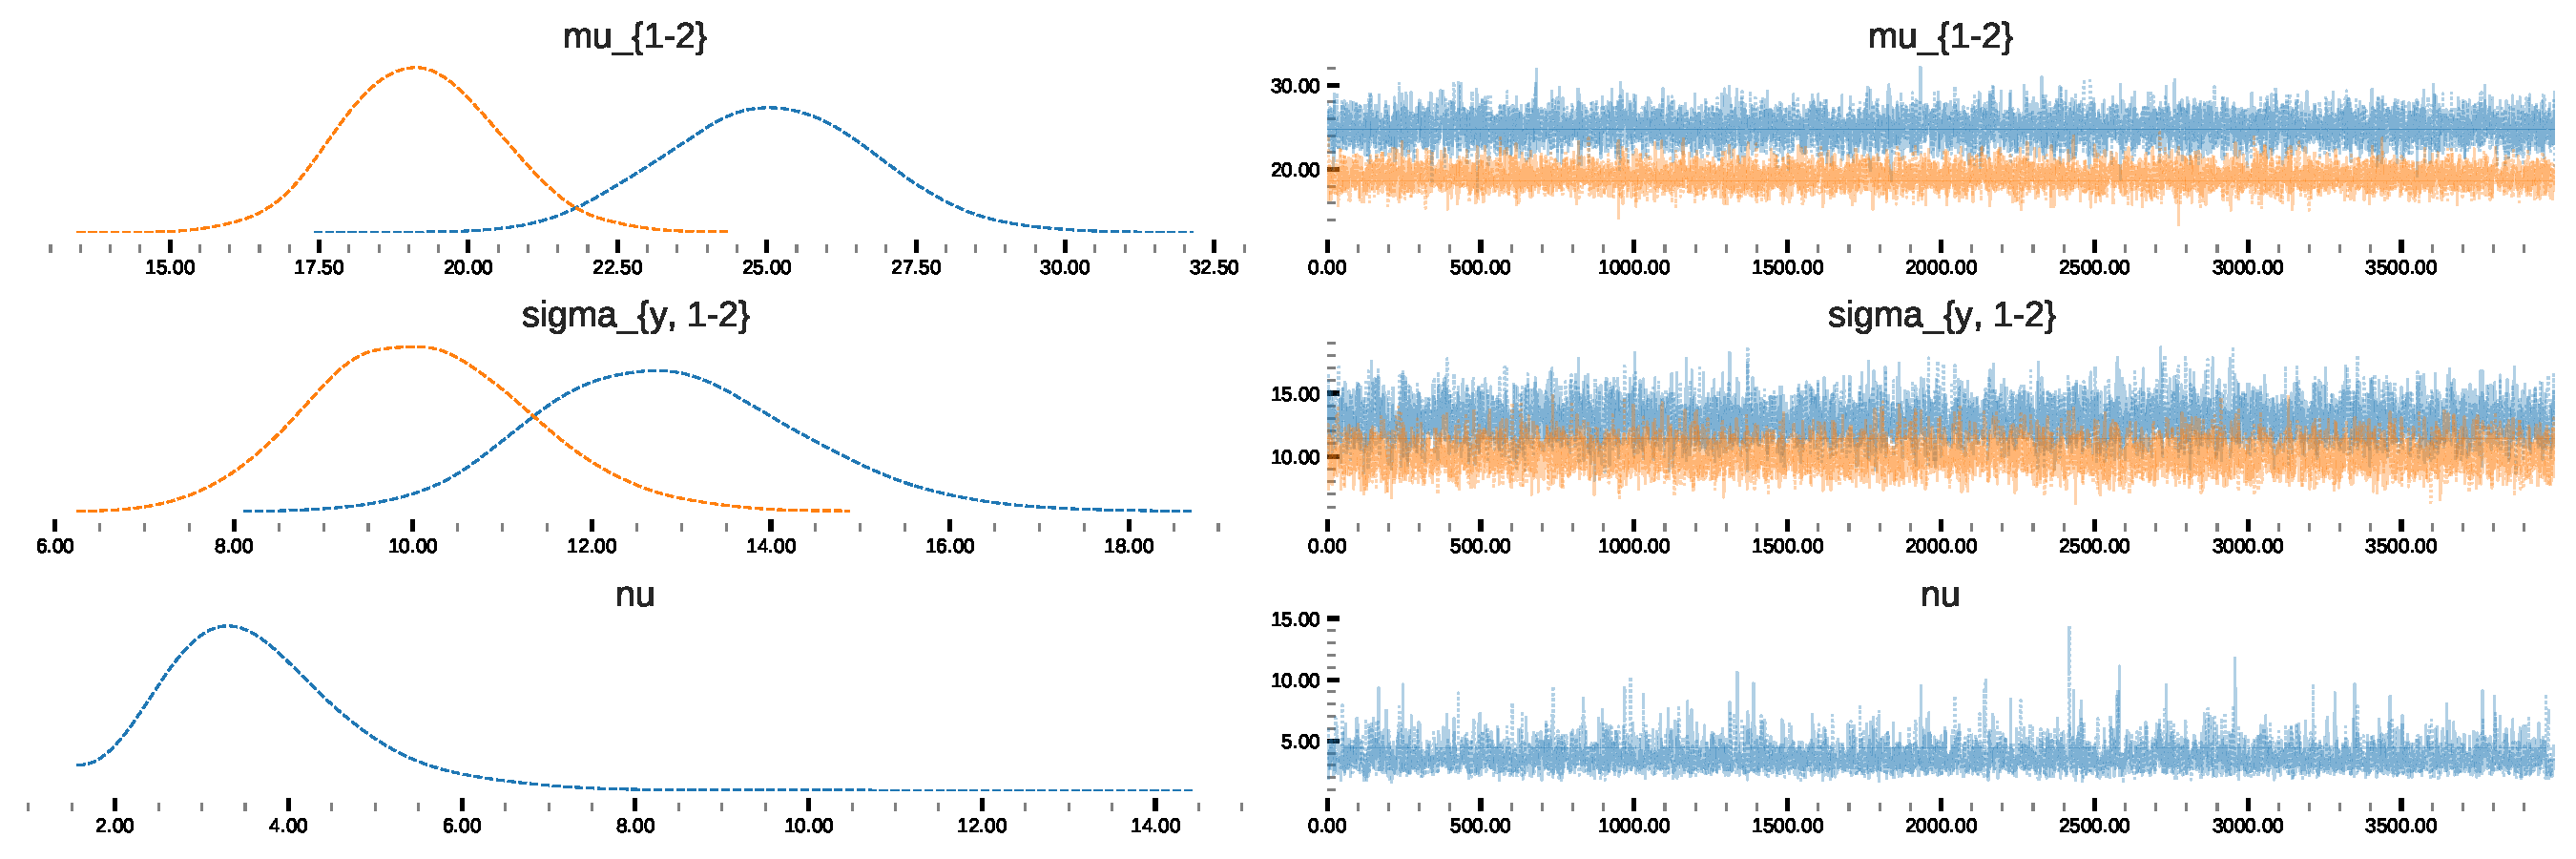
\includegraphics[trim= 0in 0in 0in 0in, clip, width=\textwidth, keepaspectratio=true]{content/image/StudentTIndep_traceplot.pdf}
  \caption{
    Traceplot showing the results of the MCMC estimation in experiment 2. The left column is the posterior distributions for $\mu_{1-2}$, $\sigma_{1-2}$, and $\nu$ of the Student-t distribution. The right column shows the corresponding sampling traces. The color mappings are: orange -- QV, blue -- Likert. Distribution for $\mu_{1-2}$ of QV is to the left of Likert, meaning a better alignment with price setting behaviors. Note also, that the modal value for degrees of freedom $\nu \approx 3$, confirming our choice of the Student-t distribution instead of the Normal distribution, which usually requires $\nu \geq 30$. Furthermore, the Gelman-Rubin statistic $\hat{R}$ for all parameters was 1, indicating  convergence of the sampling MCMC chains.
  }
  \Description[Traceplot for the MCMC estimation in experiment 2 Bayesian model]{Traceplot for the MCMC estimation in experiment 2 Bayesian model}
  \label{fig:traceplot_exp2}
\end{sidewaysfigure*}